\chapter{Metodologia}

\section{Revisão da Literatura}

Os conceitos teóricos explicados a seguir são baseados nas notas de aula, na obra de \textcite{heywood2018internal}, \textcite{blair1999design}, \textcite{ferguson2015internal}.

\subsection{Áreas}

Parâmetros geométricos são de suma importância para o motor. 
Áreas relacionadas às válvulas são necessárias para a compreensão do desempenho do motor.
Á área de cortina é a região referente à ``parede'' formada pelo levante da válvula, como mostra a~\cref{fig:area_cortina}.
A área de garganta representa a área circular da diferença entre a área do diâmetro da válvula e do diâmetro da haste, como mostra a~\cref{fig:area_garganta} influenciando a quantidade de massa fresca que entra na câmara de combustão.
A área de cortina e de garganta para cada cilindro é dada, respectivamente, por: 
%
\begin{align}
    A_c &= \pi D_v L_v
    \label{eq:area_cortina} \\
    A_g &= \frac{\pi \left(D^2_v - D^2_h\right)}{4} 
    \label{eq:area_garganta}
\end{align}
%
onde $D_v$ é o diâmetro da válvula, $L_v$ é abertura da d válvula e $D_h$ é o diâmetro da haste da válvula. 
%
\begin{figure}[!htb]
    \centering
    \begin{minipage}{0.49\textwidth}
        \centering
        \caption{Área de Cortina em uma Válvula}
        \includesvg[width=0.5\textwidth]{figuras/area_de_cortina.svg}
        \fonte{elaborado pelos autores.}
        \label{fig:area_cortina}
    \end{minipage}
    \hfill
    \begin{minipage}{0.49\textwidth}
        \centering
        \caption{Área de Garganta em uma Válvula}
        \includesvg[width=0.5\textwidth]{figuras/area_de_garganta.svg}
        \fonte{elaborado pelos autores.}
        \label{fig:area_garganta}
    \end{minipage}
\end{figure}
%
\subsection{Coeficiente de Descarga}

O coeficiente de descarga é a razão entre o fluxo de ar que está passando através do componente durante o ensaio, pelo fluxo de ar que deveria passar pelo componente durante o ensaio caso o escoamento isentrópico e é dado por:
%
\begin{equation}
    C_d = \frac{Q_r}{Q_t}
    \label{eq:coef_descarga}
\end{equation}
%
onde $Q_r$ o fluxo de massa real e $Q_t = V_{\text{th}} A$ é o fluxo de massa caso o escoamento fosse isentrópico. A velocidade de escoamento isentrópica (teórica) pode ser calculada como:
%
\begin{equation}
    V_{\text{th}} = \sqrt{\frac{P_0}{\rho_s} \cdot \frac{2\gamma}{\gamma-1} \left[1 - \left( \frac{P_0 - \Delta P}{P_0} \right)^{\frac{\gamma-1}{\gamma}}\right]}
    \label{eq:velocidade_isentropica}
\end{equation}
%
onde $P_0$ é a pressão ambiente, $\gamma = 1,4$ é o coeficiente politrópico, $\Delta P$ é a pressão de teste de bancada, e $\rho_s$ é a densidade no fluxo de ar e pode ser calculado a partir da seguinte expressão:
%
\begin{equation}
    \rho_s = \rho_0 \left( \frac{P_0 - \Delta P}{P_0} \right)^{\frac{1}{\gamma}}
\end{equation}
%
onde $\rho_0$ é a densidade do ar ambiente. A área de fluxo $A$ pode ser a área de cortina ou a área de garganta, a depender do tipo de análise. A vazão real é medida experimentalmente através de uma bancada de ensaio de fluxo. A densisdade do ar ambiente é determinada através da equação geral dos gases:
\begin{equation}
    \rho_0 = \frac{P}{R_aT}
\end{equation} 
%
onde $P$ é a pressão ambiente, $T$ é a temperatura ambiente e $R_a = \SI{287}{J.kg^{-1}.K^{-1}}$ é a constante do ar \cite{cengel2015mecanica}.

Outra abordagem para se determinar o coeficiente de descarga é utilizando a área de garganta efetiva:
%
\begin{equation}
    A_{ge} = \frac{Q_r \sqrt{\gamma R_aT}}{\gamma P_0 \left(\frac{\Delta P}{P_0}\right)^{\frac{1}{\gamma}} \sqrt{\frac{2}{\gamma-1} \left(1 - \frac{\Delta P}{P_0}\right)^{\frac{\gamma-1}{\gamma}} }}
    \label{eq:area_garganta_efetiva}
\end{equation}
%
então o coeficiente de descarga pode ser calculado como:
%
\begin{equation}
    C_d = \frac{A_{ge}}{A_g}
    \label{eq:coef_descarga_area_efetiva}
\end{equation}

\subsection{Pressão Média}

A pressão média efetiva (BMEP) é mede a eficiência do motor de combustão interna, já levando em consideração a perda de pressão por bombeamento e atrito. Ela pode ser calculada como mostra a expressão a seguir:
%
\begin{equation}
    \text{BMEP} = \frac{2 \dot{W}}{n V_d N}
    \label{eq:bmep}
\end{equation}
%
onde $\dot{W}$ é a potência do motor, $n$ é o número de cilindros, $V_d$ é o volume deslocado do pistão e $N$ é a rotação do motor.

\subsection{Carga Lateral}

A carga lateral do pistão é obtida através da análise de forças no pistão a partir das leis da mecânica dos sólidos e é dada por:
%
\begin{equation}
    F_L = \frac{\pi d P (R/L) \sin\alpha}{4\sqrt{1-(R/L)^2\sin^2\alpha}}
    \label{eq:carga_lateral}
\end{equation}
%
onde $d$ é o diâmetro do pistão, $P$ é a pressão exercida, $R$ é o comprimento da manivela, $L$ é o comprimento da biela e $\alpha$ é o ângulo percorrido pela manivela a partir do ponto morto superior (PMS).

\subsection{Velocidade do pistão}

Sabendo que a cada rotação o pistão percorre duas vezes o cilindro e que o raio da manivela vale duas vezes o curso do pistão, a velocidade média do pistão pode ser calculado como mostra a expressão a:
%
\begin{equation}
    v_m = 4NR
    \label{eq:velocidade_media}
\end{equation}

A partir de geometria simples, é possível determinar a posição do cilindro em relação ao ângulo de rotação da manivela. Sabendo que $\alpha=\omega t$, determina-se a velocidade instantânea através da derivada da posicão do cilindro:
%
\begin{equation}
    v = R\omega\sin\omega t \left( 1 + \dfrac{R\cos\omega t}{\sqrt{L^2-R^2-\sin^2\omega t}} \right)
    \label{eq:velocidade}
\end{equation}

\subsection{Número de Mach}

O número de Mach é um termo adimensional e é definido como \cite{cengel2015mecanica}:
%
\begin{equation}
    \ma = \frac{V}{c}
    \label{eq:mach}
\end{equation}
%
onde $V$ é a velocidade do escoamento e $c \approx \SI{343}{m.s^{-1}}$ é a velocidade do som. Também pode ser determinado como:
%
\begin{equation}
    \ma = \frac{\pi D v_m}{4 A_g c}
    \label{eq:mach_f}
\end{equation}

\section{Montagem Experimental}

Para o ensaio de fluxo no cabeçote, foi utilizada um bancada de ensaio fluxo, monitorada por um software próprio, com encaixe para o motor a ser utilizado, como mostra a~\cref{fig:motor_bancada}. 
Um motor EA211 TSI foi utilizado para ser acoplado na bancada.
As válvulas de escape e admissão, referentes ao motor utilizado, foram retiradas temporariamente para tomar as medidas geométricas de cada uma. As válvulas utilizadas estão representadas na~\cref{fig:valvulas}, sendo a da esquerda (menor) a válvula de escape e a da direita (maior) a válvula de admissão.
A bancada de fluxo manteve-se conectado a um computador que, através do software Servitec WinSSFluxo, monitorava o fluxo a partir das condições estabelecidas.
%
\begin{figure}[!htb]
    \centering
    \begin{minipage}[t]{0.49\textwidth}
        \centering
        \caption{Motor na Bancada de Fluxo}
        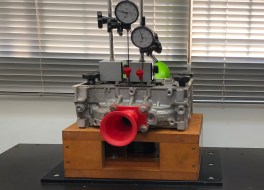
\includegraphics{figuras/motor_na_bancada.png}
        \fonte{elaborado pelos autores.}
        \label{fig:motor_bancada}
    \end{minipage}
    \hfill
    \begin{minipage}[t]{0.49\textwidth}
        \centering
        \caption{Válvulas Utilizadas} 
        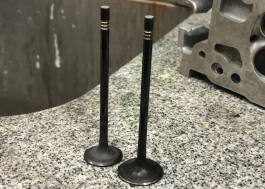
\includegraphics{figuras/valvulas.png}
        \fonte{elaborado pelos autores.}
        \label{fig:valvulas}
    \end{minipage}
\end{figure}
%
Para o ensaio dinamométrico, o motor John Deere, modelo 6068 Tier 3, mostrado na~\cref{fig:motor_jd}, foi utilizado com condição de carga de 75\%. Na sala de controle (\cref{fig:sala_controle}), foram determinadas as condições de operação e realizada a geração dos dados.
%
\begin{figure}[!htb]
    \centering
    \begin{minipage}[t]{0.49\textwidth}
        \centering
        \caption{Motor John Deere}
        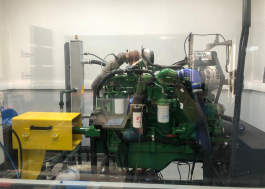
\includegraphics{figuras/motor_jd.png}
        \fonte{elaborado pelos autores.}
        \label{fig:motor_jd}
    \end{minipage}
    \hfill
    \begin{minipage}[t]{0.49\textwidth}
        \centering
        \caption{Sala de Controle}
        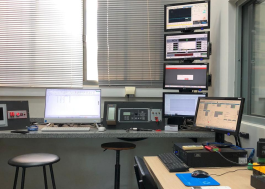
\includegraphics{figuras/sala_controle.png}
        \fonte{elaborado pelos autores.}
        \label{fig:sala_controle}
    \end{minipage}
\end{figure}
%
\section{Procedimento Experimental}

\subsection{Ensaio de Fluxo no Cabeçote}

\begin{enumerate}[label=\itshape\roman*.]
    \item Inicialmente, foram tomadas as dimensões das válvulas de admissão e escape do motor;
    \item foi realizada a calibração da bancada de ensaio de fluxo;
    \item o motor EA211 TSI foi posicionado na bancada;
    \item o ensaio foi realizado considerando admissão na válvula de admissão, em seguida exaustão na válvula de admissão e, por fim, exaustão na válvula de escape.
    \item o ensaio de fluxo foi realizado considerando a abertura da válvula entre 0 e 10 mm, com passo de 1 mm;
    \item para cada levante da válvula, foram tomadas as medidas da vazão (fluxo).
\end{enumerate}

\subsection{Ensaio Dinamométrico}

\begin{enumerate}[label=\itshape\roman*.]
    \item Na sala de controle, através do software, foram definidas as condições de operação;
    \item o motor foi ligado e acionado em diferentes rotações;
    \item diversos parâmetros foram armazenados, para cada faixa de intervalo das rotações.
\end{enumerate}
